%*******************************************************************************
%****************************** Second Chapter *********************************
%*******************************************************************************

\chapter{Resultados Capítulo 1} 
{\LARGE Estudios genómicos sobre la biogénesis de miARN en plantas}

\graphicspath{{Chapter2/Figs/}}

\section{Introducción}
Los miARNs son una clase de ARNs de 20-22nt de largo que son originados de genes endógenos y regulan otros ARNs por complementariedad de bases \citep{Voinnet2009669}.
Se distinguen de otros ARNs pequeños por su biogénesis única que involucra el corte preciso del precursor, para liberar el miARN maduro.
Aunque la evidencia actual indica que los miARNs han surgido y especializada de forma independiente en animales y las plantas, su biogénesis depende del reconocimiento de claves estructurales ubicadas en los precursores de miARN \citep{pmid21554756,citeulike:8816489,Bologna11112012}.

En nuestro grupo actualmente se está estudiando la biogenesis de miARNs, específicamente como los precursores son reconocidos y procesados en plantas \citep{Bologna2013}.
Estos precursores tienen una estructura de tallo-burbuja característica \citep{Jones-Rhoades2006}, que se cree que proporciona las claves para el procesamiento del mismo y la liberación de los ARN pequeños de 21 nt.

Mientras que los precursores de miARN en animales tienen estructuras homogéneas, los precursores de miARNs en plantas constituyen una amplia gama de estructuras, y sus longitud pueden variar entre 50 y 900 nucleótidos \citep{Bologna2013,citeulike:8816489}.
En particular, la biogénesis de los miARNs es un proceso clave porque determina la secuencia exacta de nucleótidos del ARN pequeño funcional.
Si bien en el caso de animales está claro cuáles elementos estructurales son reconocidos en los precursores durante su procesamiento, poco se sabía sobre el reconocimiento de los precursores de plantas por la maquinaria de procesamiento.

Muchos precursores en plantas tienen un tallo de $\sim$15 nt debajo del duplex miARN/miARN* seguido por un loop interno, que sirve como una señal estructural de reconocimiento por la maquinaria de procesamiento \citep{pmid17369351,pmid16751099,Mateos2010,pmid20015654}.
Sin embargo, este determinante de procesamiento no se encuentra en todos los precursores \citep{Mateos2010}.
Además, la biogénesis de los miARNs conservados evolutivamente como ser el miR319 y miR159 comienzan con un corte al lado del loop interno y continúa con 3 cortes adicionales en una dirección de burbuja a base hasta que finalmente el miARN es liberado \citep{Bologna2013,pmid19850910}.
Se ha demostrado que otros precursores de plantas liberan otros ARNs pequeños además del miARN \citep{pmid15314213,pmid20696037}, aunque los mecanismos de procesamiento subyacentes eran desconocidos.

\section{Resultados} 

\subsection{Procesamiento de precursores de miARNs en plantas}

En esta parte del proyecto de tesis y en el marco de una colaboración con el grupo del Dr. Blake Meyers (Delaware,USA), el cual se especializa en secuenciación y análisis de ARN pequeños, nos propusimos entender cómo se procesan los precursores de miARNs plantas. 
Colegas del laboratorio realizaron una estrategia para analizar sistemáticamente intermediarios de procesamiento de miARNs y caracterizar la biogénesis de la mayoría de los miARNs conservados presentes en Arabidopsis thaliana mediante técnicas de secuenciación de alto rendimiento, utilizando los equipos de última generación disponibles en Delaware (USA).
Esta técnica desarrollada en el laboratorio se conoce como sPARE \citep{Schapire2013} (del inglés Specific Parallel Amplification of RNA Ends).
Utilizando esta técnica encontramos que los miARNs son procesados por cuatro mecanismos, dependientes de la dirección secuencial de la maquinaria de procesamiento y del número de cortes requeridos para liberar el miARN.
La clasificación de los precursores, teniendo en cuenta los mecanismos de procesamiento, reveló determinantes estructurales específicos para cada grupo.
Se encontró que la complejidad de las vías de procesamiento de miARN se produce tanto en precursores jóvenes como en conservados y que los miembros de la misma familia pueden ser procesados de diferentes maneras.
Además hemos observado que diferentes determinantes estructurales compiten por la maquinaria de procesamiento y que miRNAs alternativos pueden ser generados a partir de un único precursor.
Los resultados ofrecen una explicación para la diversidad estructural de los genes de precursores de miARN en plantas y nuevas perspectivas hacia la comprensión de la biogénesis de los ARNs pequeños \citep{Bologna2013}.


\subsubsection{Análisis de datos y precursores detectados}
Mediante la cantidad de cortes detectados la técnica de sPARE permite definir si el mecanismo es base a loop o loop a base.
Esta técnica arroja una gran cantidad de datos producto de la secuenciación de alto rendimiento, por lo que se necesita de un enfoque bioinformático para la interpretación de los resultados.
Por la gran cantidad de precursores a estudiar y el número de bibliotecas se necesitó un análisis previo de los datos y una forma de presentarlos.
Para esto construimos e implementamos un pipeline bioinformático utilizando "in-house" scripts y datos disponibles de miRBASE para poder analizar los datos de las bibliotecas de deep-sequencing obtenidos a partir de la técnica de SPARE.

Un precursor fue considerado como detectado si más de tres lecturas corresponden a la secuencia de ese precursor.
De esta manera encontramos fragmentos de ARN que corresponden a 129 precursores, 71 de ellos de miARNs conservados y 58 de miARNs jóvenes (Figura \ref{fig:GR_fig1C}).
Mediante el análisis de los datos arrojados de la estrategia bioinformática pudimos definir la dirección de procesamiento de la mayoría de los precursores en \textit{A. thaliana}.
De los cuales 32 de ellos fueron definidos como procesados por un mecanismo de base a loop, ya que se encontraron los cortes en la parte proximal del duplex miARN/miARN* sin detectar cortes en la parte de arriba del duplex, como en el caso del miR168a, miR172b y el miR395b (Figura \ref{fig:GR_fig2A}).
Además encontramos 16 precursores de miARNs conservados con cortes detectados (>5\%) en el lado distal del miARN/miARN* los cuales fueron definidos como loop a base (Figura \ref{fig:GR_fig4A}).

\begin{figure}[htbp!] 
    \centering    
    \includegraphics[width=.5\textwidth]{GR_fig1C.png}
    \caption[Esquema del procedimiento para analizar los datos de sPARE]{Esquema del procedimiento para analizar los datos de sPARE.}
    \label{fig:GR_fig1C}
\end{figure}

\begin{figure}[htbp!] 
    \centering    
    \includegraphics[width=1\textwidth]{GR_fig2A.png}
    \caption[Identificación y caracterización de precursores de miARNs procesados de base a loop]{Identificación y caracterización de precursores de miARNs procesados de base a loop.
            Esquema donde se muestra la estructura secundaria del miR168a, miR172b y miR395b.
            Las flechas indican la posición y número de lecturas de los cortes del precursor identificado.
            Flechas en verde muestra el corte más abundante, que también coincide con al corte proximal del miARN/miARN*.
            Flechas en negro muestran otros cortes con al menos 5\% de abundancia del número total de cortes, mientras que otros cortes minoritarios se muestran con una flecha gris.
            Con rosa se resalta el stem de 15nt debajo del corte proximal.
            El miARN se indica en color rojo y el miARN* en color azul.
            La imagen de la derecha muestra el patrón de corte típico detectado en la biblioteca de sPARE para estos precursores.}
    \label{fig:GR_fig2A}
\end{figure}


\begin{figure}[htbp!] 
    \centering    
    \includegraphics[width=1\textwidth]{GR_fig4A.png}
    \caption[Identificación y caracterización de precursores de miARNs procesados de loop a base]{Identificación y caracterización de precursores de miARNs procesados de loop a base. 
    Esquema donde se muestra la estructura secundaria del miR156a, miR156c, miR156d y miR160a.
    Las flechas indican la posición y número de lecturas de los cortes del precursor identificado.
    Flechas en verde muestra el corte más abundante, que también coincide con al corte proximal del miARN/miARN*.
    Flechas en negro muestran otros cortes con al menos 5\% de abundancia del número total de cortes, mientras que otros cortes minoritarios se muestran con una flecha gris.
    Con gris se resalta el stem de arriba del miR156 y miR160. El miARN se indica en color rojo y el miARN* en color azul.
    La imagen de la derecha muestra el patrón de corte típico detectado en la biblioteca de SPARE para estos precursores.
}
    \label{fig:GR_fig4A}
\end{figure}

\subsubsection{Estructura secundaria de los precursores}
Para ver si había diferencias estructurales para los precursores con diferentes mecanismos de procesamiento, determinamos la estructura secundaria de precursores detectados que se procesan en dirección base a loop (Figura \ref{fig:GR_fig2C}) y los que se procesan loop a base (Figura \ref{fig:GR_fig4C}).
Obtuvimos las estructuras secundarias para cada precursor.
Definimos a una coincidencia en cada posición con un 0, mientras que bulges y mismatches los consideramos como 1.
El lado proximal del duplex miARN/miARN* fue definido como la posición +1 y analizamos desde la posición -25 a la posición +40 (Figura \ref{fig:GR_fig2C} y \ref{fig:GR_fig4C}). 

\subsubsection{Procesamiento de base a loop}

Consideramos la estructura secundaria de 32 precursores analizados en esta parte del trabajo que se procesan de base a loop y todos ellos tienen un claro tallo inferior de 15 nt de largo (Figura \ref{fig:GR_fig2C}).
Además este tallo se pudo ver tanto para los precursores validados experimentalmente que se procesan de base a loop como para todos los precursores conservados (Figura \ref{fig:GR_fig2C} en violeta).
Pero pudimos observar que las bases inmediatamente debajo del duplex miARN/miARN* (posición -2 y -1) tienden a estar desapareadas (Figura \ref{fig:GR_fig2C}).
Además las posiciones -3 y -4 y las 3 últimas posiciones del stem inferior (-13,-14 y -15) están apareadas casi siempre (Figura \ref{fig:GR_fig2C}).
En general, nuestros resultados muestran que los precursores procesados en una dirección base a loop son más uniformes de lo que se pensaba previamente y que al menos algunos de los precursores no detectados como base a loop probablemente tengan otros determinantes específicos de ARN.

\subsubsection{Procesamiento de loop a base}
Estos precursores, que tienen un procesamiento loop a base, tienen un corte mayoritario que se puede detectar en nuestras bibliotecas.
Este corte es el esperado en la dirección de procesamiento de precursores con un mecanismo de loop a base.
Con la excepción de dos miARNs (miR396a y miR162b) estos precursores no tienen una estructura obvia debajo del duplex miARN/miARN* (Figura \ref{fig:GR_fig4C}).
Estos precursores tienen una región terminal estructurada (Figura \ref{fig:GR_fig4C}), que tiene un tamaño homogéneo de ~42nt que incluye un loop corto en contraste con la misma región en los precursores que se procesan de base a loop donde es más variable (Figura \ref{fig:GR_fig2C} y \ref{fig:GR_fig4C}). 

En esta segunda parte del proyecto de tesis presentamos un estrategia y realizamos un análisis sistemático para la identificación de la biogénesis de precursores de miARNs desde un punto de vista genómico.
De esta manera pudimos encontrar la dirección de procesamiento de la mayoría de los precursores de miARNs en \textit{A. thaliana}.

\begin{figure}[htbp!] 
    \centering    
    \includegraphics[width=1\textwidth]{GR_fig2C.png}
    \caption[Estructura secundaria de precursores de base a loop]{Estructura secundaria de precursores detectados que se procesan en dirección base a loop.
    Los matches en cada posición los consideramos como 0, mientras que bulges y mismatches fueron considerados como 1.
    La estructura secundaria considerando todos los miARNs conservados se indica con color violeta.
    }
    \label{fig:GR_fig2C}
\end{figure}

\begin{figure}[htbp!] 
    \centering    
    \includegraphics[width=1\textwidth]{GR_fig4C.png}
    \caption[Estructura secundaria de precursores de loop a base]{
    Estructura secundaria de precursores detectados que se procesan en dirección loop a base.
    Los matches en cada posición los consideramos como 0, mientras que bulges y mismatches fueron considerados como 1.}
    \label{fig:GR_fig4C}
\end{figure}


Estos resultados fueron publicado en la revista Genome Research \citep{Bologna2013}.
Em este mismo artículo se pudo demostrar que los precursores de miARNs en plantas, se pueden agrupar por cuatro mecanismos de procesamiento con distintas características (Figura \ref{fig:mecanismos}).

\begin{itemize}
    \item En los precursores con un mecanismo \textbf{corto de base a loop}, un loop interno seguido por un tallo inferior de $\sim$15nt especifica la posición del primer corte.
        Esta estructura se encuentra en la mayoría de familias de miARNs \citep{Mateos2010,pmid20015653,pmid20015654}.
        A pesar de que el tallo puede contener bulges, la transición de un loop interno (simple hebra) al tallo inferior es bastante marcada, y tres pares de bases apareadas generalmente definen el comienzo del tallo inferior del precursor \citep{Bologna2013}.
        El segundo corte procede a una distancia fija de $\sim$21 nt desde la posición del primer corte.
    \item En los precursores con un mecanismo \textbf{secuencial de base a loop} (ej: familia del miR169), el primer corte procede como en los cortos de base a loop, pero luego son necesario dos cortes más para liberar el miARN, generando en el proceso niveles bajos de RNA pequeños adicionales \citep{Bologna2013}.
    \item En los precursores con un mecanismo \textbf{cortos de loop a base} (ej: familia del miR156 y miR160), el procesamiento es guiado por un tallo superior, y son necesarios dos cortes para liberar el miARN maduro.
        La región terminal de estos precursores tienen una largo conservado de $\sim$42 y un loop pequeño \citep{Bologna2013}.
    \item En los precursores con un mecanismo \textbf{secuencial de loop a base} (ej: familia del miR319 y miR159), cuatro cortes secuenciales por DCL1 son los encargados de procesar los precursores de miARNs.
        En general muestran un tallo largo superior, del cual otros ARNs pequeños son generados \citep{pmid19850910,Bologna2009,Bologna2013}
\end{itemize}

\begin{figure}[htbp!] 
    \centering    
    \includegraphics[width=1\textwidth]{mecanismos.png}
    \caption[Mecanismos de procesamiento]{Distintos mecanismos de procesamientos de miARNs en plantas}
    \label{fig:mecanismos}
\end{figure}


Que los precursores de miARNs en plantas sean procesados de diferentes maneras, nos llevó a especular que su patrón de evolución también puede ser diferente y podrían estar vinculados a su mecanismo de procesamiento.


\subsection{Enfoque bioinformático para el estudio de la evolución y biogénesis de miARNs en plantas}


%~ Estudios recientes del laboratorio revelaron que en plantas los precursores de miARNs pueden procesarse por al menos cuatro mecanismos diferentes \citep{Bologna2013}, indicando que la diversidad de estructuras secundaria podría correlacionar con el mecanismo de biogénesis de los miARNs. 

